\subsection {Unpacking raw data from the camera}
\label{sec:unpacking}
The first step in the transformation process is to unpack the raw data from the camera.
The \lucid cameras feature a 12-bit \gls{adc} and offer 23 different output formats with varying bit depths and packing.
As the \gls{h265} encoder supports 10-bit data, the \code{Mono10p} output format was chosen for the cameras \cite[17 ]{nvidiaNVIDIAJetsonAGX2019}.
This format densly packs the 10-bit data, as depicted in Figure \ref{fig:mono10p}, maximizing the network throughput.

\begin{figure}[H]
    \centering
    \subcaptionbox{Pixel data.}{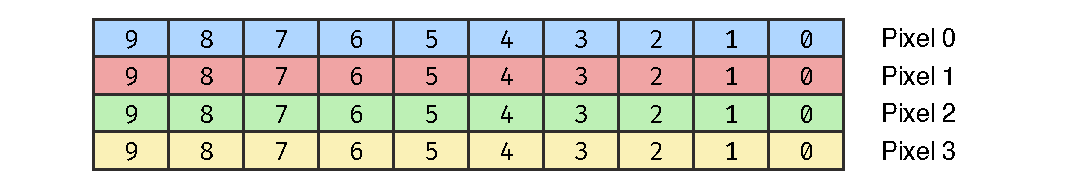
\includegraphics[width=\textwidth]{figures/unpacking/layout_10p.pdf}}
    \subcaptionbox{Bytes sent over ethernet.}{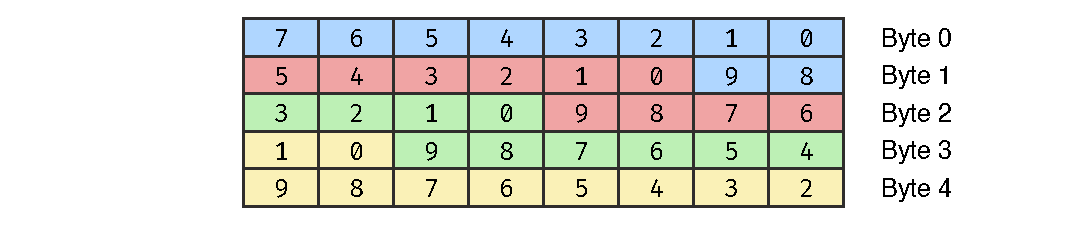
\includegraphics[width=\textwidth]{figures/unpacking/layout_10p_sent.pdf}}
    \caption{Bit layout of the \code{Mono10p} format.}
    \label{fig:mono10p}
\end{figure}

I encountered difficulties in locating documentation regarding the bit ordering on Lucid's website.
As a workaround, I relied on two test images provided by the \cam.
These test images contained pixel values that increased monotonically, as depicted in Figure \ref{fig:test_pattern}.
By analyzing the data in the first line in these images, I was able to deduce the bit ordering.
Regrettably, I later discovered that Lucid Vision does provide separate documentation on pixel formats; however, it did not appear in their own search engine for unknown reasons \cite{lucidvisionlabsPixelFormatsLUCID2020}.

\begin{figure}[H]
    \centering
    
\includegraphics[width=0.4\textwidth]{figures/unpacking/test_pattern0.jpg}
    
\includegraphics[width=0.4\textwidth]{figures/unpacking/test_pattern2.jpg}
    \caption{Two test images used to infer the bit ordering.
        The \cam can output several different test patterns useful for various testing purposes \cite{lucidvisionlabsTritonMPPolarized2020}.}
    \label{fig:test_pattern}
\end{figure}


\subsubsection{Bit unpacking} \label{sec:contuguous_access}
The pattern in Figure \ref{fig:mono10p} was identified as representing an little endian unsigned integer.
By reordering the bytes vuisually the bit pattern in Figure \ref{fig:mono10p} becomes more intuitive, as shown in Figure \ref{fig:mono10p_reordered}.

\begin{figure}[H]
    \centering
    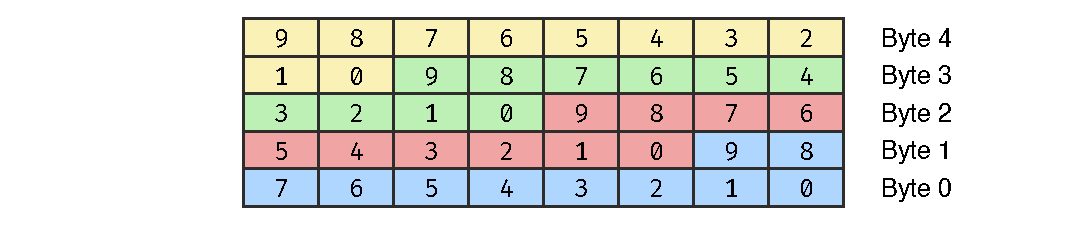
\includegraphics[width=\textwidth]{figures/unpacking/layout_10p_be.pdf}
    \caption{More intuitive visualization of the bit ordering in Figure \ref{fig:test_pattern}.}
    \label{fig:mono10p_reordered}
\end{figure}

As the CUDA GPU architecture uses little-endian representation this is beneficial as we can interpred the incoming bits as a sequence of word sized (32-bit) unsigned integers directly \cite[127]{CUDAProgrammingGuide}.
The first three pixel values are then read as from the 30 least significant bits of the first word, the fourth pixel value is read from the most significant bits of the first word and the least 8 significant bits of the secont word and so on.
This can be extracted using bit manipulation as shown in Listing \ref{lst:unpacking}.
To get proper byte alignment each thread unpacks 5 words (160 bits), which corresponds to 16 pixel values.

\begin{listing}[H]
    \begin{minted}{cuda}
        word_a = data[idx];
        word_b = data[idx+1];
        vals[0] = word_a & 0b1111111111;
        vals[1] = word_a >> 10 & 0b1111111111;
        vals[2] = word_a >> 20 & 0b1111111111;
        vals[3] = word_a >> 30 & 0b11 | (word_b & 0b11111111) << 2;
        vals[4] = word_b >> 8 & 0b1111111111;
        vals[5] = word_b >> 18 & 0b1111111111;
    \end{minted}
    \caption{Psuedo code showing how the first six pixel values are unpacked.}
    \label{lst:unpacking}
\end{listing}


